\begin{blocksection}
\question 
Solve for the maximum controller overhead to meet the following specifications: We need disk latency under 18 ms while reading 800 B of data.  The hard drive spins at 6000 rev/min with a seek time of 2.5 ms and transfer rate of 80 KB/s (SI prefix).  Don’t forget units!
\begin{solution}[0.5in] 
0.5 ms \\
controller overhead $\leq$ disk latency – seek time – rotation time – transfer time \\
rotation time = 0.5/rpm * (60 sec/1 min) = 0.005 s = 5 ms \\
transfer time = data size/transfer rate = 0.01 s = 10 ms \\
controller overhead $\leq$ 18 – 2.5 – 5 – 10 ms = 0.5 ms\\
\end{solution}

\question
To support interrupts, the CPU should be able to save and restore the current state. Which of the following should be saved before handling interrupts to ensure correct execution? \\
a. Program Counter 	b. User Registers 	c. TLB 		d. Caches
\begin{solution}[0.5in] 
b \\
The PC gets saved to track where to return to after handling the interrupt. Similarly, the User Registers save information about the state before the interrupt. These are necessary to ensure correct execution. However, the TLB and Caches are implemented for efficiency, so execution would still be correct without them.
\end{solution}

\question
Consider the following three devices. For which device is Direct Memory Access (DMA) most beneficial?\\

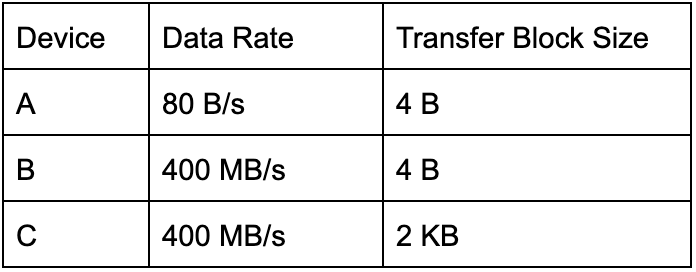
\includegraphics[width=\textwidth]{io/devices}
\begin{solution}[0.5in] 
Device C. \\
DMA allows us to transfer data to/from memory independent of the CPU. This will be most useful when we have to write or read a lot of data from memory, as that will free up the most time for the processor to perform other tasks. Since C has the largest data block, it will receive the most benefit from DMA.     
\end{solution}

\end{blocksection}